\documentclass[aspectratio=169]{beamer}
\usepackage{booktabs}
\usepackage{graphicx}
\usepackage{adjustbox}
\usepackage{amsmath}
% xcolor and define colors -------------------------
\usepackage{xcolor}

% https://www.viget.com/articles/color-contrast/
\definecolor{purple}{HTML}{695693}
\definecolor{navy}{HTML}{567293}
\definecolor{ruby}{HTML}{9a2515}
\definecolor{alice}{HTML}{107895}
\definecolor{daisy}{HTML}{EBC944}
\definecolor{coral}{HTML}{F26D21}
\definecolor{kelly}{HTML}{829356}
\definecolor{cranberry}{HTML}{E64173}
\definecolor{jet}{HTML}{131516}
\definecolor{asher}{HTML}{555F61}
\definecolor{slate}{HTML}{314F4F}

% Main theme colors
\definecolor{accent}{HTML}{107895}
\definecolor{accent2}{HTML}{9a2515}

\newcommand\navy[1]{{\color{navy}#1}}
\newcommand\purple[1]{{\color{purple}#1}}
\newcommand\kelly[1]{{\color{kelly}#1}}
\newcommand\ruby[1]{{\color{ruby}#1}}
\newcommand\alice[1]{{\color{alice}#1}}
\newcommand\daisy[1]{{\color{daisy}#1}}
\newcommand\coral[1]{{\color{coral}#1}}
\newcommand\cranberry[1]{{\color{cranberry}#1}}
\newcommand\slate[1]{{\color{slate}#1}}
\newcommand\jet[1]{{\color{jet}#1}}
\newcommand\asher[1]{{\color{asher}#1}}

\newcommand\bgNavy[1]{{\colorbox{navy!80!white}{\textcolor{white}{#1}}}}
\newcommand\bgPurple[1]{{\colorbox{purple!80!white}{\textcolor{white}{#1}}}}
\newcommand\bgKelly[1]{{\colorbox{kelly!80!white}{\textcolor{white}{#1}}}}
\newcommand\bgRuby[1]{{\colorbox{ruby!80!white}{\textcolor{white}{#1}}}}
\newcommand\bgAlice[1]{{\colorbox{alice!80!white}{\textcolor{white}{#1}}}}
\newcommand\bgDaisy[1]{{\colorbox{daisy!80!white}{\textcolor{white}{#1}}}}
\newcommand\bgCoral[1]{{\colorbox{coral!80!white}{\textcolor{white}{#1}}}}
\newcommand\bgCranberry[1]{{\colorbox{cranberry!80!white}{\textcolor{white}{#1}}}}


% Beamer Options -------------------------------------

% Background
\setbeamercolor{background canvas}{bg = white}

% Change text margins
\setbeamersize{text margin left = 15pt, text margin right = 15pt} 

% \alert
\setbeamercolor{alerted text}{fg = accent2}

% Frame title
\setbeamercolor{frametitle}{bg = white, fg = jet}
\setbeamercolor{framesubtitle}{bg = white, fg = accent}
\setbeamerfont{framesubtitle}{size = \small, shape = \itshape}

% Block
\setbeamercolor{block title}{fg = white, bg = accent2}
\setbeamercolor{block body}{fg = jet, bg = jet!10!white}

% Title page
\setbeamercolor{title}{fg = jet}
\setbeamercolor{subtitle}{fg = accent}

%% Custom \maketitle and \titlepage
\setbeamertemplate{title page}
{
    %\begin{centering}
        \vspace{20mm}
        {\Large \usebeamerfont{title}\usebeamercolor[fg]{title}\inserttitle}\\ \vskip0.25em%
        \ifx\insertsubtitle\@empty%
        \else%
          {\usebeamerfont{subtitle}\usebeamercolor[fg]{subtitle}\insertsubtitle\par}%
        \fi% 
        {\vspace{10mm}\insertauthor}\\
        {\color{asher}\small{\insertdate}}\\
    %\end{centering}
}

% Table of Contents
\setbeamercolor{section in toc}{fg = accent!70!jet}
\setbeamercolor{subsection in toc}{fg = jet}

% Button 
\setbeamercolor{button}{bg = accent}

% Remove navigation symbols
\setbeamertemplate{navigation symbols}{}

% Optional: page numbers at bottom
\addtobeamertemplate{navigation symbols}{}{%
    \usebeamerfont{footline}%
    \hspace{1em}%
    \alice{\insertframenumber/\inserttotalframenumber}
    \vspace*{1.5mm}
}


% Table and Figure captions
\setbeamercolor{caption}{fg=jet!70!white}
\setbeamercolor{caption name}{fg=jet}
\setbeamerfont{caption name}{shape = \itshape}

% Bullet points

%% Fix left-margins
\settowidth{\leftmargini}{\usebeamertemplate{itemize item}}
\addtolength{\leftmargini}{\labelsep}

%% enumerate item color
\setbeamercolor{enumerate item}{fg = accent}
\setbeamerfont{enumerate item}{size = \small}
\setbeamertemplate{enumerate item}{\insertenumlabel.}

%% enumerate subitem color
\setbeamercolor{enumerate subitem}{fg = accent!60!white}
\setbeamerfont{enumerate subitem}{size = \small}
\setbeamertemplate{enumerate subitem}{\insertenumlabel.}

%% itemize
\setbeamercolor{itemize item}{fg = accent!70!white}
\setbeamerfont{itemize item}{size = \small}
\setbeamertemplate{itemize item}[circle]

%% right arrow for subitems
\setbeamercolor{itemize subitem}{fg = accent!60!white}
\setbeamerfont{itemize subitem}{size = \small}
\setbeamertemplate{itemize subitem}{$\rightarrow$}

\setbeamertemplate{itemize subsubitem}[square]
\setbeamercolor{itemize subsubitem}{fg = jet}
\setbeamerfont{itemize subsubitem}{size = \small}

% References

%% Bibliography Font, roughly matching aea
\setbeamerfont{bibliography item}{size = \footnotesize}
\setbeamerfont{bibliography entry author}{size = \footnotesize, series = \bfseries}
\setbeamerfont{bibliography entry title}{size = \footnotesize}
\setbeamerfont{bibliography entry location}{size = \footnotesize, shape = \itshape}
\setbeamerfont{bibliography entry note}{size = \footnotesize}

\setbeamercolor{bibliography item}{fg = jet}
\setbeamercolor{bibliography entry author}{fg = accent!60!jet}
\setbeamercolor{bibliography entry title}{fg = jet}
\setbeamercolor{bibliography entry location}{fg = jet}
\setbeamercolor{bibliography entry note}{fg = jet}

%% Remove bibliography symbol in slides
\setbeamertemplate{bibliography item}{}





% Links ----------------------------------------------

\usepackage{hyperref}
\hypersetup{
  colorlinks = true,
  linkcolor = accent2,
  filecolor = accent2,
  urlcolor = accent2,
  citecolor = accent2,
}


% Line spacing --------------------------------------
\usepackage{setspace}
% \setdisplayskipstretch{2}
\setstretch{1.3}


% \begin{columns} -----------------------------------
\usepackage{multicol}


% Fonts ---------------------------------------------
% Beamer Option to use custom fonts
\usefonttheme{professionalfonts}

% \usepackage[utopia, smallerops, varg]{newtxmath}
% \usepackage{utopia}
\usepackage[sfdefault,light]{roboto}

% Small adjustments to text kerning
\usepackage{microtype}



% Remove annoying over-full box warnings -----------
\vfuzz2pt 
\hfuzz2pt


% Table of Contents with Sections
\setbeamerfont{myTOC}{series=\bfseries, size=\Large}
\AtBeginSection[]{
        \frame{
            \frametitle{Roadmap}
            \tableofcontents[current]   
        }
    }


% References ----------------------------------------
\usepackage[
    citestyle= authoryear,
    style = authoryear,
    natbib = true, 
    backend = biber
]{biblatex}

% Smaller font-size for references
\renewcommand*{\bibfont}{\small}

% Remove "In:"
\renewbibmacro{in:}{}

% Color citations for slides
\newenvironment{citecolor}
    {\footnotesize\begin{color}{accent2}}
    {\end{color}}

\newcommand{\citetcolor}[1]{{\footnotesize\textcolor{gray}{\citet{#1}}}}
\newcommand{\citepcolor}[1]{{\footnotesize\textcolor{gray}{\citep{#1}}}}

% Tables -------------------------------------------
% Tables too big
% \begin{adjustbox}{width = 1.2\textwidth, center}
\usepackage{adjustbox}
\usepackage{array}
\usepackage{threeparttable, booktabs, adjustbox}
    
% Fix \input with tables
% \input fails when \\ is at end of external .tex file

\makeatletter
\let\input\@@input
\makeatother

% Tables too narrow
% \begin{tabularx}{\linewidth}{cols}
% col-types: X - center, L - left, R -right
% Relative scale: >{\hsize=.8\hsize}X/L/R
\usepackage{tabularx}
\newcolumntype{L}{>{\raggedright\arraybackslash}X}
\newcolumntype{R}{>{\raggedleft\arraybackslash}X}
\newcolumntype{C}{>{\centering\arraybackslash}X}

% Figures

% \imageframe{img_name} -----------------------------
% from https://github.com/mattjetwell/cousteau
\newcommand{\imageframe}[1]{%
    \begin{frame}[plain]
        \begin{tikzpicture}[remember picture, overlay]
            \node[at = (current page.center), xshift = 0cm] (cover) {%
                \includegraphics[keepaspectratio, width=\paperwidth, height=\paperheight]{#1}
            };
        \end{tikzpicture}
    \end{frame}%
}

% subfigures
\usepackage{subfigure}

% Strikeout text
\usepackage{cancel}

% Highlight slide -----------------------------------
% \begin{transitionframe} Text \end{transitionframe}
% from paulgp's beamer tips
\newenvironment{transitionframe}{
    \setbeamercolor{background canvas}{bg=accent!60!black}
    \begin{frame}\color{accent!10!white}\LARGE\centering
}{
    \end{frame}
}


% Table Highlighting --------------------------------
% Create top-left and bottom-right markets in tabular cells with a unique matching id and these commands will outline those cells
\usepackage[beamer,customcolors]{hf-tikz}
\usetikzlibrary{calc,fit,shapes.misc,backgrounds}
\usepackage{pgfplots}
\pgfplotsset{compat = newest}
\usetikzlibrary{positioning, arrows.meta}
\usepgfplotslibrary{fillbetween}

% halo around text
%https://tex.stackexchange.com/questions/18472/tikz-halo-around-text
\usepackage[outline]{contour} 
\contourlength{1.2pt}
\tikzset{
  contour text/.style={node contents={\contour{white}{#1}}},
  halo text node/.style={circle, draw, pattern=north east lines}
}


\def\arraystretch{0.75}

% To set the hypothesis highlighting boxes red.
\newcommand\marktopleft[1]{%
    \tikz[overlay,remember picture] 
        \node (marker-#1-a) at (0,1.5ex) {};%
}
\newcommand\markbottomright[1]{%
    \tikz[overlay,remember picture] 
        \node (marker-#1-b) at (0,0) {};%
    \tikz[accent!80!jet, ultra thick, overlay, remember picture, inner sep=4pt]
        \node[draw, rectangle, fit=(marker-#1-a.center) (marker-#1-b.center)] {};%
}


\author{Michael R. Karas}
\title{Math Review}
\subtitle{ECON 3070 - Intermediate Microeconomic Theory}
\date{January X, 2025}

\begin{document}

% ------------------------------------------------------------------------------------------------
\begin{frame}
  \titlepage
\end{frame}
% ------------------------------------------------------------------------------------------------

% ------------------------------------------------------------------------------------------------
\begin{frame}{Math Review Topics}\label{main1}
\begin{itemize}
	\begin{itemize}
		\item Limits
		\item Derivative Definition
		\item Derivative Rules
		\item Partial Derivatives
	\end{itemize}
\end{itemize}

\end{frame}
% ------------------------------------------------------------------------------------------------

% ------------------------------------------------------------------------------------------------
\begin{frame}{Limits}\label{main1}
	The limit of \( f(x) \) as \( x \) approaches \( a \) is written as:
\[
\lim_{x \to a} f(x)
\]
\begin{itemize}
\begin{itemize}
	\item The behavior of the function as its input approaches \( a \)
	\item In certain cases, can be evaluated by plugging in \( x = a \)
	\item \( \lim_{x \to a} c = c \) for a constant \( c \)
	\item \(\lim_{x \to a} x = a \) for a constant \( c \)
\end{itemize}
\end{itemize}

\end{frame}
% ------------------------------------------------------------------------------------------------

% ------------------------------------------------------------------------------------------------
\begin{frame}{Limits}\label{main1}
The limit from the left and right are
\begin{itemize}
\begin{itemize}
    \item \(\lim_{x \to a^-} f(x) = A\) “as \(x\) approaches \(a\) from the left (\(-\infty\))”
    \item \(\lim_{x \to a^+} f(x) = A\) “as \(x\) approaches \(a\) from the right (\(\infty\))”
\end{itemize}
\end{itemize}
If \(\lim_{x \to a^-} f(x) = A = \lim_{x \to a^+} f(x)\) then the limit exists and we write
\[
\lim_{x \to a} f(x) = A
\]
\begin{itemize}
    \item Note: the limit does not exist if \(A = \pm\infty\), even if the left and right limit both equal \(\pm\infty\)
\end{itemize}
\end{frame}
% ------------------------------------------------------------------------------------------------

% ------------------------------------------------------------------------------------------------
\begin{frame}{Limits}\label{main1}
    \begin{figure}
        \centering
        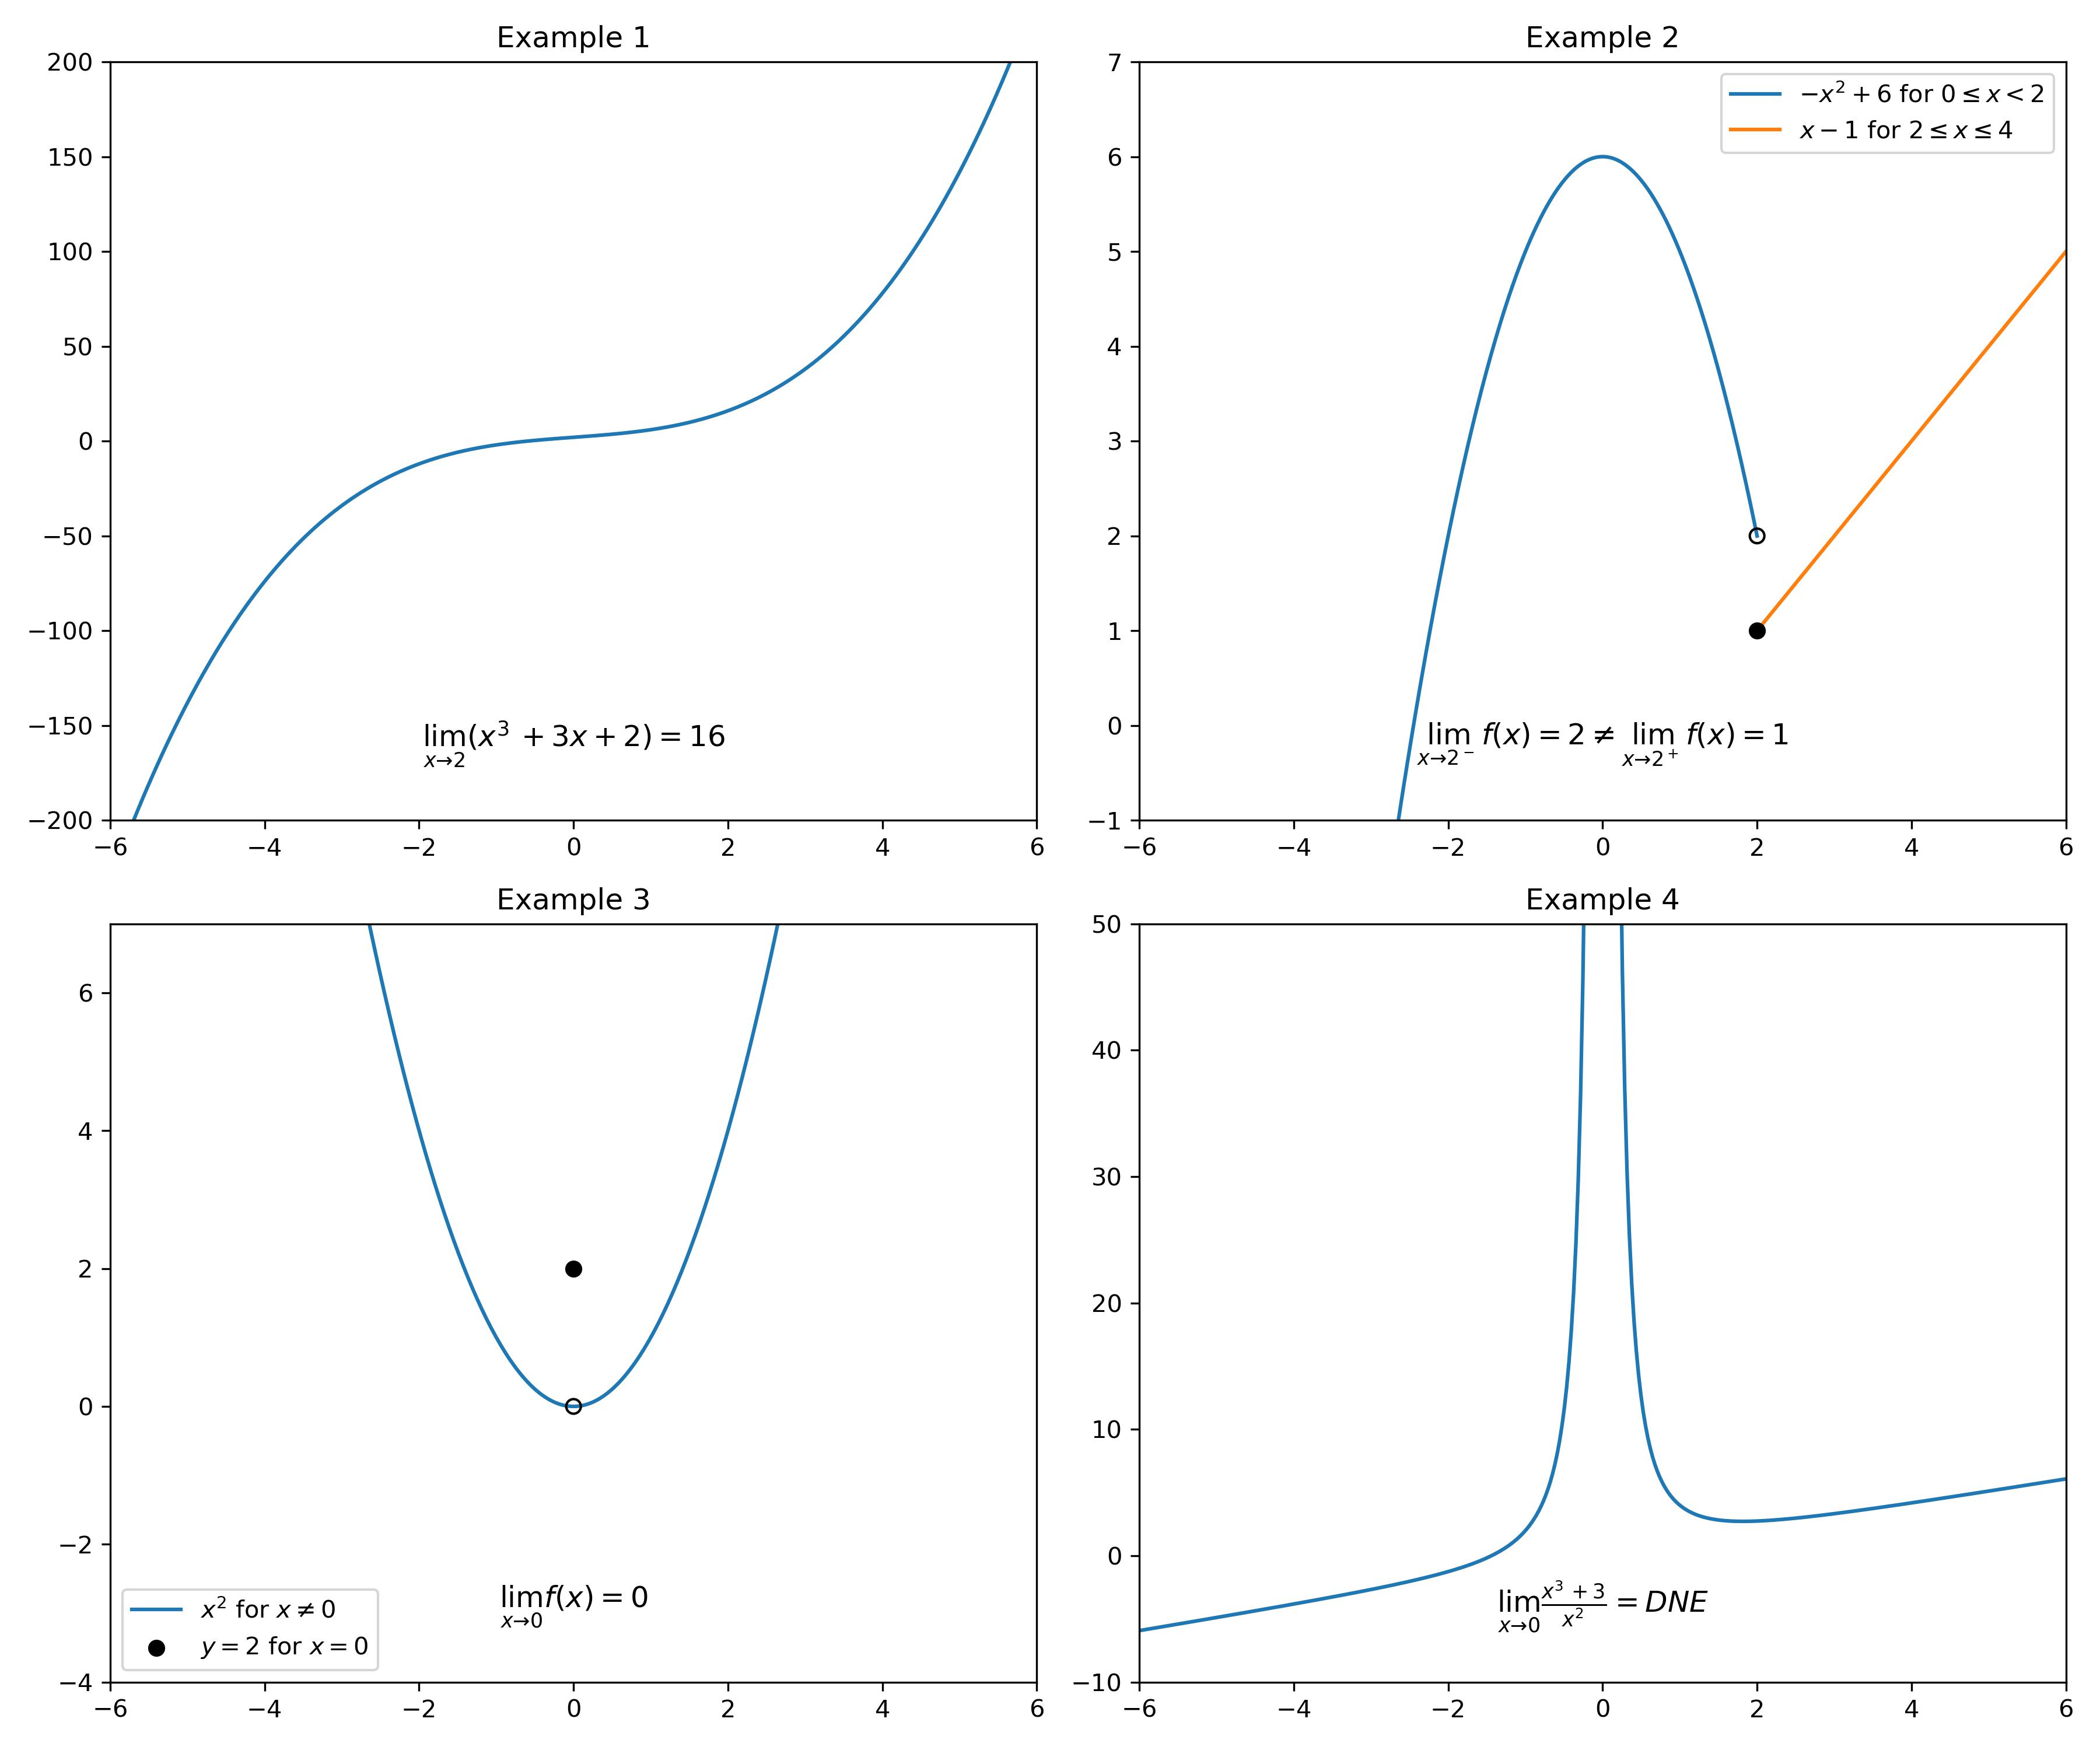
\includegraphics[width=0.75\textwidth]{figures/limits_example.jpg}
    \end{figure}
\end{frame}
% ------------------------------------------------------------------------------------------------

% ------------------------------------------------------------------------------------------------
\begin{frame}{Limit Rules}\label{main1}
    \[
    \lim_{x \to a} f(x) = L \quad \lim_{x \to a} g(x) = M
    \]
    \vspace{1em}
    \begin{itemize}
        \item \textbf{Constant Multiple Rule:} \quad $\lim_{x \to a} [a f(x)] = a L$
        \item \textbf{Sum/Difference Rule:} \quad $\lim_{x \to a} [f(x) \pm g(x)] = L \pm M$
        \item \textbf{Product Rule:} \quad $\lim_{x \to a} [f(x) \cdot g(x)] = L \cdot M$
        \item \textbf{Quotient Rule:} \quad $\lim_{x \to a} \left[ \frac{f(x)}{g(x)} \right] = \frac{L}{M}, \quad M \neq 0$
        \item \textbf{Power Rule:} \quad $\lim_{x \to a} [(f(x))^n] = L^n, \quad n > 0$
    \end{itemize}
\end{frame}
% ------------------------------------------------------------------------------------------------

% ------------------------------------------------------------------------------------------------
\begin{frame}{Definition of a Derivative}\label{main1}
The derivative of \(f\) is defined as
\[
f'(x) = \lim_{h \to 0} \frac{f(x + h) - f(x)}{h}
\]
If this limit exists, then we say \(f\) is differentiable at \(x\).

\end{frame}
% ------------------------------------------------------------------------------------------------

% ------------------------------------------------------------------------------------------------
\begin{frame}{Derivative Notation}\label{main1}
All of these mean “take the derivative of \(f\) with respect to \(x\)”:
\begin{itemize}
\begin{itemize}
    \item \(f'(x)\)
    \item \(\frac{df(x)}{dx}\)
    \item \(\frac{d}{dx} f(x)\)
    \item \(\frac{dy}{dx}\) if \(y = f(x)\)
    \item \(y'\) (sometimes)
    \item \( \dot{y} \) (particularly in Macro)
\end{itemize}
\end{itemize}
\end{frame}
% ------------------------------------------------------------------------------------------------

% ------------------------------------------------------------------------------------------------
\begin{frame}{Derivative Rules}\label{main1}
Let \(f(x)\) and \(g(x)\) be differentiable functions:
\begin{itemize}
    \item \textbf{Derivative of a Constant:} \(f(x) = c\), \(f'(x) = 0\)
    \item \textbf{“Power Rule”:} \(f(x) = x^n\), \(f'(x) = nx^{n-1}\) 
    \item \textbf{Sum/Difference Rule:} \quad $\frac{d}{dx} [f(x) \pm g(x)] = f'(x) \pm g'(x)$
    \item \textbf{Product Rule:} \quad $\frac{d}{dx} [f(x) \cdot g(x)] = f'(x) \cdot g(x) + f(x) \cdot g'(x)$
    \item \textbf{Quotient Rule:} \quad $\frac{d}{dx} \left( \frac{f(x)}{g(x)} \right) = \frac{f'(x) \cdot g(x) - f(x) \cdot g'(x)}{[g(x)]^2}$
    \item \textbf{Chain Rule:} \quad $\frac{d}{dx} f(g(x)) = f'(g(x)) \cdot g'(x)$
\end{itemize}
\end{frame}
% ------------------------------------------------------------------------------------------------

% ------------------------------------------------------------------------------------------------
\begin{frame}{Derivatives Practice Problems}\label{main1}
	\vspace{-4cm}
     \[
    f(x) = 2x
    \]
\end{frame}
% ------------------------------------------------------------------------------------------------

% ------------------------------------------------------------------------------------------------
\begin{frame}{Derivatives Practice Problems}\label{main1}
	\vspace{-4cm}
     \[
    f(x) = 3x^2
    \]
\end{frame}
% ------------------------------------------------------------------------------------------------

% ------------------------------------------------------------------------------------------------
\begin{frame}{Derivative Rules for Exponents and Natural Log}\label{main1}
\begin{itemize}
\begin{itemize}
    \item \(f(x) = e^x\), \(f'(x) = e^x\)
    \item \(f(x) = \ln(x)\), \(f'(x) = \frac{1}{x}\)
\end{itemize}
\end{itemize}
\bigskip
Useful review of the properties of \hyperlink{exponentslide}{exponents} and \hyperlink{naturallogslide}{logs}.
\end{frame}
% ------------------------------------------------------------------------------------------------

% ------------------------------------------------------------------------------------------------
\begin{frame}{Derivatives Practice Problems}\label{main1}
	\vspace{-4cm}
     \[
    f(x) = ln(e^x)
    \]
\end{frame}
% ------------------------------------------------------------------------------------------------

% ------------------------------------------------------------------------------------------------
\begin{frame}{Derivatives Practice Problems}\label{main1}
	\vspace{-4cm}
     \[
    f(x) = x^{2}ln(x)
    \]
\end{frame}
% ------------------------------------------------------------------------------------------------

% ------------------------------------------------------------------------------------------------
\begin{frame}{Derivatives Practice Problems}\label{main1}
	\vspace{-4cm}
     \[
    f(x) = e^{2x}
    \]
\end{frame}
% ------------------------------------------------------------------------------------------------

% ------------------------------------------------------------------------------------------------
\begin{frame}{Higher-order Derivatives}\label{main1}
The second-order derivative is

\[
f''(x) = \frac{d}{dx} f'(x)
\]

We could keep differentiating as long as the last derivative is differentiable. Notation:
\begin{itemize}
\begin{itemize}
    \item $f''(x)$
    \item $\frac{d^2 f(x)}{dx^2}$
    \item $\frac{d^2}{dx^2} f(x)$
    \item $\frac{d^2 y}{dx^2}$ if $y = f(x)$
    \item $y''$ (sometimes)
\end{itemize}
\end{itemize}
\end{frame}
% ------------------------------------------------------------------------------------------------

% ------------------------------------------------------------------------------------------------
\begin{frame}{Partial Derivatives}\label{main1}
    The function $z = f(x, y)$ takes two inputs and outputs a third.  We can evaluate what happens to that output when we change $x$ or $y$ (but not both).
    \begin{itemize}
        \item $\frac{\partial z}{\partial x} =$ “the derivative of $z$ with respect to $x$”
        \begin{itemize}
        \item The slope of $f$ in the cardinal direction of $x$ (e.g. “north-south”)
        \item The tangent of $f$ in the $x$ direction at a point $(x_0, y_0)$
        \end{itemize}
        \item $\frac{\partial z}{\partial y} =$ “the derivative of $z$ with respect to $y$”
        \begin{itemize}
        \item The slope of $f$ in the cardinal direction of $y$ (e.g. “east-west”)
        \item The tangent of $f$ in the $y$ direction at a point $(x_0, y_0)$
    	\end{itemize}
    \end{itemize}
\end{frame}
% ------------------------------------------------------------------------------------------------

% ------------------------------------------------------------------------------------------------
\begin{frame}{Partial Derivatives}\label{main1}
    All of these mean “take the partial derivative of $f$ with respect to $x$”:
    \begin{itemize}
        \item $f_x(x, y)$
        \item $\frac{\partial f(x, y)}{\partial x}$
        \item $\frac{\partial}{\partial x} f(x, y)$
        \item $\frac{\partial z}{\partial x}$ if $z = f(x, y)$
    \end{itemize}
\end{frame}
% ------------------------------------------------------------------------------------------------

% ------------------------------------------------------------------------------------------------
\begin{frame}{Partial Derivatives}\label{main1}
    Interpret $\frac{\partial z}{\partial x}$ as “what happens to $z$ if I change $x$, holding $y$ constant.” Likewise for $\frac{\partial z}{\partial y}$.
 	Suppose $z = x + y + xy$, find $\frac{\partial z}{\partial x}$.
    \[
    \frac{\partial z}{\partial x} = \frac{\partial}{\partial x} [x + y + xy] = \frac{\partial}{\partial x} x + \frac{\partial}{\partial x} y + \frac{\partial}{\partial x} xy = 1 + 0 + y \cdot 1 = 1 + y
    \]
\end{frame}
% ------------------------------------------------------------------------------------------------

% ------------------------------------------------------------------------------------------------
\begin{frame}{Partial Derivatives Practice Problems}\label{main1}
	\vspace{-4cm}
     \[
    f(x,y) = x^{2} + y^{2} + x^{2}y^{2}
    \]
\end{frame}
% ------------------------------------------------------------------------------------------------

% ------------------------------------------------------------------------------------------------
\begin{frame}{Partial Derivatives Practice Problems}\label{main1}
	\vspace{-4cm}
     \[
    f(x,y) = x^{2}y+ln(x)y^{3}
    \]
\end{frame}
% ------------------------------------------------------------------------------------------------

% ------------------------------------------------------------------------------------------------
\begin{frame}{Properties of Exponents}\label{main1}
\hypertarget{exponentslide}{}
Let $a$ and $b$ be real numbers and $m$ and $n$ be integers. Then the following properties of exponents hold, provided that all of the expressions appearing in a particular equation are defined:
\begin{itemize}
\begin{itemize}
    \item $a^m a^n = a^{m+n}$
    \item $(a^m)^n = a^{mn}$
    \item $(ab)^m = a^m b^m$
    \item $\frac{a^m}{a^n} = a^{m-n}$, $a \neq 0$
    \item $\left(\frac{a}{b}\right)^m = \frac{a^m}{b^m}$, $b \neq 0$
    \item $a^{-m} = \frac{1}{a^m}$, $a \neq 0$
    \item $a^{\frac{1}{n}} = \sqrt[n]{a}$
    \item $a^0 = 1$, $a \neq 0$
    \item $a^{\frac{m}{n}} = \sqrt[n]{a^m} = \left(\sqrt[n]{a}\right)^m$
\end{itemize}
\end{itemize}
\end{frame}
% ------------------------------------------------------------------------------------------------

% ------------------------------------------------------------------------------------------------
\begin{frame}{Properties of Natural Log}\label{main1}
\hypertarget{naturallogslide}{}
Note that logs are only defined for positive values of x:
\begin{itemize}
\begin{itemize}
    \item $\ln(xy) = \ln(x) + \ln(y)$
    \item $\ln\left(\frac{x}{y}\right) = \ln(x) - \ln(y)$
    \item $\ln(x^y) = y \cdot \ln(x)$
    \item $\ln(e^x) = x$
    \item $e^{\ln(x)} = x$
    \item $\ln(e) = 1$
    \item $\ln(1) = 0$
    \item $\ln(1) = undefined$
\end{itemize}
\end{itemize}
\end{frame}
% ------------------------------------------------------------------------------------------------

\end{document}